\section{States}
One of the data sections of a compiled model is \textit{states}.
States is a section that is reserved on the SRAMs and used as a buffer for the accumulation of the activation data of layers.
At initialization and for every new frame, the values in the states section will be set to a static value (called bias).
Before every new frame, the bias values are recomputed/initialized by the system.
Therefore, we do not need to transfer the states from the external memory.
% The accumulated values are computed as follows:
% \begin{equation*}
%     (\textrm{weight} \times \textrm{input}) + \textrm{bias}
% \end{equation*}

% For every new frame, the states section is initialized with a static set of bias values.
% This initialization process does not retrieve the bias values from the external memory but...
% \todo[inline]{Insert more explanation about states}

Since the states do not have to be read during configuration, we can improve the energy consumption by avoiding the reading of the states.
This allows us to read less data from the external memory, reducing the energy for configuration.
Furthermore, since less data is transferred, also the configuration latency should be improved.

We perform an analysis on various models to get an idea of how much we can benefit with avoiding the read of states.
The compiler provides us with the amount of bytes used for the states and other components of each model.

\begin{table}[hbtp]
\centering
\begin{tabular}{@{}lll@{}}
\toprule
\textbf{Model}          & \textbf{States ratio} & \textbf{Prune ratio} \\ \midrule
efficientnet            & 23\%                  & 20\%                 \\
mobnetv2                & 31\%                  & 0\%                  \\
object\_tracker         & 28\%                  & 20\%                 \\
object\_detector        & 51\%                  & 0\%                  \\
resnet50                & 28\%                  & 80\%                 \\
resnet101\_p0           & 24\%                  & 0\%                  \\
resnet101\_p1           & 14\%                  & 0\%                  \\
resnet101\_p2           & 15\%                  & 0\%                  \\
resnet101\_p3           & 8\%                   & 0\%                  \\
resnet101\_p4           & 6\%                   & 0\%                  \\
resnet101\_pruned\_p0   & 44\%                  & 80\%                 \\
resnet101\_pruned\_p1   & 27\%                  & 80\%                 \\
resnet101\_pruned\_p2   & 28\%                  & 80\%                 \\
resnet101\_pruned\_p3   & 14\%                  & 80\%                 \\
resnet101\_pruned\_p4   & 11\%                  & 80\%                 \\ \bottomrule
\end{tabular}
\caption{
    Ratio of the states data compared to the total mapped model data.
    All model shown are 8-bit quantized
}
\label{tab:states_ratio}
\end{table}

Looking at \cref{tab:states_ratio}, on average, $23\%$ is used for states section.
We observe that the states ratio can reach half of the total bytes to be written to the \graicore{}.
In certain cases, the states section can occupy up to half of all the data sections combined.
% Thus, with the models in \cref{tab:states_ratio}, we can reduce the amount of data to be read from the external memory by up to a half.

In terms of energy savings, the ResNet-50 model sees a decrease of 23\% in configuration energy when avoiding the reads of states from the external memory (see \cref{fig:resnet50_states_comparison}).

\begin{figure}[hbtp]
    \centering
    \subcaptionbox{Includes states}{
        \def\printonlylargeenough#1#2{{\unless\ifdim#2pt<#1pt\relax
#2\printnumbertrue
\else
\printnumberfalse
\fi}}
\newif\ifprintnumber

\begin{tikzpicture}
    \pie[
        radius=2.5,
        text=pin,
        hide number,
    ]{
        1.0/1.0\%,
        13.9/13.9\%,
        4.0/4.0\%,
        2.4/2.4\%
    }
    \pie[
        radius=2.5,
        hide number,
        color={gray, bluehue2, bluehue4, bluehue6},
        before number=\printonlylargeenough{2},
        after number=\ifprintnumber\%\fi
    ]{
        1.0/,
        13.9/,
        4.0/,
        2.4/
    }
    \pie[
        radius=2,
        text=inside,
        color={blue!60, red!60},
    ]{
        21.3/$\econf$,
        78.7/$\eproc$
    }
\end{tikzpicture}
    }
    \hfill
    \subcaptionbox*{}[0em]{
        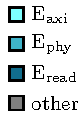
\includegraphics{assets/legend.pdf}
    }
    \hfill
    \subcaptionbox{Excludes states}{
        \def\printonlylargeenough#1#2{{\unless\ifdim#2pt<#1pt\relax
#2\printnumbertrue
\else
\printnumberfalse
\fi}}
\newif\ifprintnumber

\begin{tikzpicture}
    \pie[
        radius=2.5,
        text=pin,
        hide number,
    ]{
        0.7/0.7\%,
        10.7/10.7\%,
        3.1/3.1\%,
        1.9/1.9\%
    }
    \pie[
        radius=2.5,
        hide number,
        color={gray, bluehue2, bluehue4, bluehue6},
        before number=\printonlylargeenough{2},
        after number=\ifprintnumber\%\fi
    ]{
        0.7/,
        10.7/,
        3.1/,
        1.9/
    }
    \pie[
        radius=2,
        text=inside,
        color={blue!60, red!60},
    ]{
        16.3/$\econf$,
        83.7/$\eproc$
    }
\end{tikzpicture}
    }
    \caption{ResNet-50 states. Using LPDDR5X memory.}
    \label{fig:resnet50_states_comparison}
\end{figure}